\documentclass[tikz,convert={outfile=\jobname.svg}]{standalone}
%\documentclass{article}
%\documentclass[crop,tikz,convert={outext=.svg,command=\unexpanded{pdf2svg \infile\space\outfile}},multi=false]{standalone}[2012/04/13]
%\usetikzlibrary{...}% tikz package already loaded by 'tikz' option
%\makeatletter

%\usepackage[paperheight=4in,paperwidth=4in,margin=0in]{geometry}

%\usepackage{tikz} % already loaded
\usetikzlibrary{bayesnet}
\usetikzlibrary{shapes.geometric} % needed for squares
%\usetikzlibrary{external}
%\tikzexternalize

\usepackage{graphics}
%\pgfrealjobname{survey}
%pdflatex --jobname=ordinalModel1 graphicalModels.tex

\newcommand{\Irater}{r}
\newcommand{\Iitem}{i}
\newcommand{\Ipatient}{p}
\newcommand{\Incat}{c}

\newcommand{\Trater}{\expandafter\MakeUppercase\expandafter{\Irater}}
\newcommand{\Titem}{\expandafter\MakeUppercase\expandafter{\Iitem}}
\newcommand{\Tpatient}{\expandafter\MakeUppercase\expandafter{\Ipatient}}
\newcommand{\Tncat}{\expandafter\MakeUppercase\expandafter{\Incat}}

\tikzstyle{obs} = [square,fill=gray!25,draw=black,inner sep=1pt,minimum size=20pt, font=\fontsize{10}{10}\selectfont, node distance=1]

\begin{document}
%\beginpgfgraphicnamed{ordinalModel1}
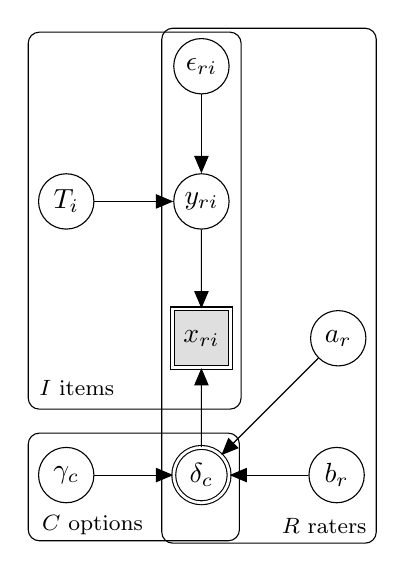
\begin{tikzpicture}[square/.style={regular polygon,regular polygon sides=4}]
%\draw [help lines] (-3,-5) grid (3,5);			

% Define nodes
\node[obs, double distance=1pt]                         (x)   {$x_{\Irater\Iitem}$};
\node[latent, below = of x, double distance = 1pt]      (d) {$\delta_\Incat$};
\node[latent, right = of x]                             (a)      {$a_\Irater$};
\node[latent, right = of d]                             (b)      {$b_\Irater$};
\node[latent, left  = of d]                             (g) {$\gamma_\Incat$};

\node[latent, above = of x]                             (y) {$y_{\Irater\Iitem}$};
\node[latent, above = of y]                             (e) {$\epsilon_{\Irater\Iitem}$};
\node[latent, left  = of y]                             (t) {$T_\Iitem$};

% Edges
\edge {d}       {x};%
\edge {a, b, g} {d};%
\edge {t, e}    {y};%
\edge {y}       {x};%

\plate[text centered] {ni} {(a)(b)(d)(x)(y)(e)}     {$\Trater$ raters };
{\tikzset{plate caption/.append style={below=4pt of #1.south west, xshift = .5cm}}
\plate[text centered, yshift = -.05cm] {ni} {(t)(x)(y)(e)}            {$\Titem$ items  };
}
{\tikzset{plate caption/.append style={below=4pt of #1.south west, xshift = .7cm}}
\plate[text centered, yshift =  .05cm] {nc} {(g)(d)}              {$\Tncat$ options};
}
\end{tikzpicture}
%\endpgfgraphicnamed
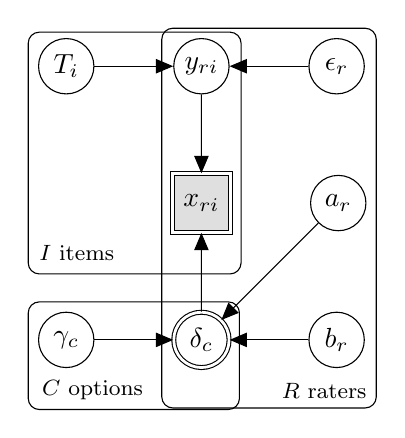
\begin{tikzpicture}[square/.style={regular polygon,regular polygon sides=4}]
%\draw [help lines] (-3,-5) grid (3,5);			

%\def\xshift{0.7cm}
%\def\plateX{.42cm}
%\def\hab{2.81cm}
%
%\def\distxnD{1.5cm}

% Define nodes
\node[obs, double distance=1pt]                         (x)   {$x_{\Irater\Iitem}$};
\node[latent, below = of x, double distance = 1pt]      (d) {$\delta_\Incat$};
\node[latent, right = of x]                             (a)      {$a_\Irater$};
\node[latent, right = of d]                             (b)      {$b_\Irater$};
\node[latent, left  = of d]                             (g) {$\gamma_\Incat$};

\node[latent, above = of x]                             (y) {$y_{\Irater\Iitem}$};
\node[latent, right = of y]                             (e) {$\epsilon_{\Irater}$};
\node[latent, left  = of y]                             (t) {$T_\Iitem$};

% Edges
\edge {d}       {x};%
\edge {a, b, g} {d};%
\edge {t, e}    {y};%
\edge {y}       {x};%

\plate[text centered] {ni} {(a)(b)(d)(x)(y)}     {$\Trater$ raters };
{\tikzset{plate caption/.append style={below=4pt of #1.south west, xshift = .5cm}}
	\plate[text centered, yshift = -.05cm] {ni} {(t)(x)(y)}            {$\Titem$ items  };
}
{\tikzset{plate caption/.append style={below=4pt of #1.south west, xshift = .7cm}}
	\plate[text centered] {nc} {(g)(d)}              {$\Tncat$ options};
}
\end{tikzpicture}
%\endpgfgraphicnamed
\end{document}


